\chapter{Testowanie systemu}

Testowanie napisanej aplikacji będzie polegać na ręcznym wprowadzeniu wybranych zdjęć do systemu.
Wszystkie zdjęcia twarzy, użyte do testowania aplikacji, zostały pobrane ze zbioru CelebA~\cite{microsoft-2020-celeb1m}.
Wybrane zdjęcia (rysunek~\ref{fig:zdjeciadotestow}) zostały podzielone na dwie kategorie:

\begin{itemize}
    \item zdjęcia, które trafią do systemu jako wzorzec,
    \item zdjęcia, które zostaną wykorzystane w celu zbadania zachowania oraz trafności
    komunikatów zwracanych przez system.
\end{itemize}

\begin{figure}[H]
    \centering
    \includegraphicswithborder{images/zdjeciadotestow}
    \caption{Użyte zdjęcia do przetestowania systemu. Obok każdej grupy przedstawiona jest etykieta zdjęć.}
    \customsource
    \label{fig:zdjeciadotestow}
\end{figure}

\pagebreak


\section{Wgranie zdjęć do systemu}

Aplikacja udostępnia dla administratorów panel, za pomocą którego jest możliwe wprowadzenie
zdjęć do systemu z poziomu przeglądarki.
Po zalogowaniu się zostały wprowadzone wyżej przedstawione zdjęcia (rysunek~\ref{fig:zdjeciadotestow}).
Dla etykiety oznaczonej numerem jeden zostało wprowadzone jedno zdjęcie,
oznaczonej numerem dwa - dwa zdjęcia przedstawiające tę samą osobę, dla kolejnej trzy.
Podgląd wprowadzonych zdjęć oraz wykadrowanych twarzy został przedstawiony na rysunku~\ref{fig:po_wprowadzeniu}.

\begin{figure}[H]
    \centering
    \includegraphicswithborder{images/po_wprowadzeniu}
    \caption{ Podgląd wprowadzonych zdjęć do systemu. }
    \customsource
    \label{fig:po_wprowadzeniu}
\end{figure}

\pagebreak


\section{Zdjęcie niezawierające twarzy}

Po wysłaniu zdjęcia na serwer, zgodnie ze schematem przedstawionym na rysunku~\ref{fig:schemat_blokowy_systemu},
pierwszym krokiem jest kadrowanie twarzy.
Informacja na temat samego kadrowania nie jest znana użytkownikowi końcowemu, natomiast w przypadku,
gdy zostanie wysłane zdjęcie niezawierające twarzy, to użytkownik powinien dostać informację zwrotną.
W celu sprawdzenia, czy funkcjonalność zadziała prawidłowo, zostało wysłane na serwer zdjęcie, które zawiera krajobraz.
Z powodu, że na zdjęciu nie ma przedstawionych żadnych osób, system powinien zwrócić informację o błędzie.
Wynik testu został pokazany na rysunku~\ref{fig:wprowadzona_natura}.
Komunikat o braku twarzy został zwrócony, co oznacza, że system zachował się poprawnie.

\begin{figure}[H]
    \centering
    \includegraphicswithborder{images/wprowadzona_natura}
    \caption{ Zachowanie systemu po wprowadzeniu zdjęcia niezawierającego twarzy. }
    \customsource
    \label{fig:wprowadzona_natura}
\end{figure}


\section{Zdjęcie osoby nieznanej systemowi}

Kolejnym krokiem do przetestowania jest sprawdzenie czy system zwróci informację,
gdy zostanie wysłane zdjęcie osoby, która nie została wcześniej zaimportowana.
Z tego powodu system powinien zwrócić informację, że nie rozpoznano osoby na zdjęciu.
W tym celu zostały przygotowane zdjęcia mężczyzn oznaczone etykietą ``4'' oraz ``5'' (rysunek~\ref{fig:zdjeciadotestow}).
Wyniki testu zostały przedstawione na rysunku~\ref{fig:rezultat_nieznane}.
Dla każdego ze zdjęć został zwrócony komunikat z informacją, że nie rozpoznano osoby na zdjęciu.
Oznacza to, że system zachował się poprawnie i test można uznać za zaliczony.

\begin{figure}[]
    \centering
    \includegraphicswithborder{images/rezultat_nieznane}
    \caption{ Zachowanie systemu po wybraniu zdjęć nieznanych systemowi }
    \customsource
    \label{fig:rezultat_nieznane}
\end{figure}


\section{Zdjęcie osoby znanej systemowi}

Ostatnim krokiem w procesie jest klasyfikacja,
czyli zwrócenie informacji kto został przedstawiony na przesłanym zdjęciu.
W celu dokładniejszego przetestowania napisanej funkcjonalności specjalnie
w tym celu zostały wgrane do systemu zdjęcia osób
o różnej liczbie (rysunek~\ref{fig:po_wprowadzeniu}),
aby sprawdzić, czy wpłynie to na otrzymane wyniki.
Wyniki testu zostały przedstawione na rysunku~\ref{fig:rezultat_znane}.
Komunikaty zwrócone przez system dla zdjęć reprezentujących etykiety ``2'' oraz ``3'' są poprawne.
Dla jednego ze zdjęć przedstawiających osobę o etykiecie ``1'' system zwrócił informacje,
że nie rozpoznano osoby na zdjęciu.
\textbf{Najprawdopodobniej} spowodowane jest to tym, że w systemie znajduje się
tylko \textbf{jedno} zdjęcie reprezentujące etykietę ``1'' przedstawiające kobietę o ciemnym kolorze włosów,
a zdjęcie, dla którego system zwrócił błędny komunikat, przedstawia tę samą kobietę, tylko że w innym kolorze włosów.
Dodatkowo zdjęcie twarzy zrobione jest z inne profilu,
częściowo zasłoniętego przez włosy (rysunek~\ref{fig:porownanie_etykiety_1}).

\pagebreak

\begin{figure}[H]
    \centering
    \includegraphicswithborder{images/rezulat_znane}
    \caption{
        Zwrócone komunikaty dla wybranych zdjęć.
        Obok komunikatu została przedstawiona etykieta, którą powinien zwrócić system.
    }
    \customsource
    \label{fig:rezultat_znane}
\end{figure}


\begin{figure}[H]
    \centering
    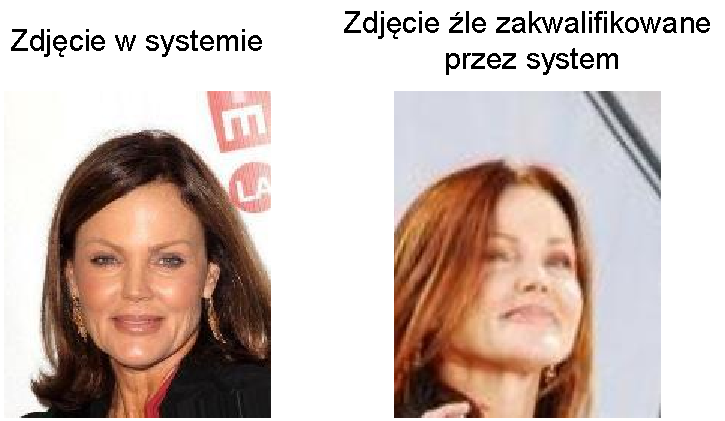
\includegraphics[width=0.6\textwidth]{images/porownanie_etykiety_1}
    \caption{ Porównanie zdjęcia wgranego do systemu ze zdjęciem źle zakwalifikowanym przez system. }
    \customsource
    \label{fig:porownanie_etykiety_1}
\end{figure}

